%
% File: chap02.tex
%
\let\textcircled=\pgftextcircled
\chapter{Results}
\label{chap:result}

\initial{I}n this section, the prompt neutron lifetime, the negative temperature coefficient and the specific heat of the core will be measured and compared to the approximate values usually used. The results are based on the data given by the computer for the power as a function of time and the fuel temperature.

\section{Results}

The higher the prompt reactivity inserted, the higher the peak power and the thinner its distribution. Figure~\ref{fig:power} shows the pulse for various insertion of positive reactivity, with a maximum peak power obtained of 1.2 GW.

\begin{figure}[t!]
	\centering
	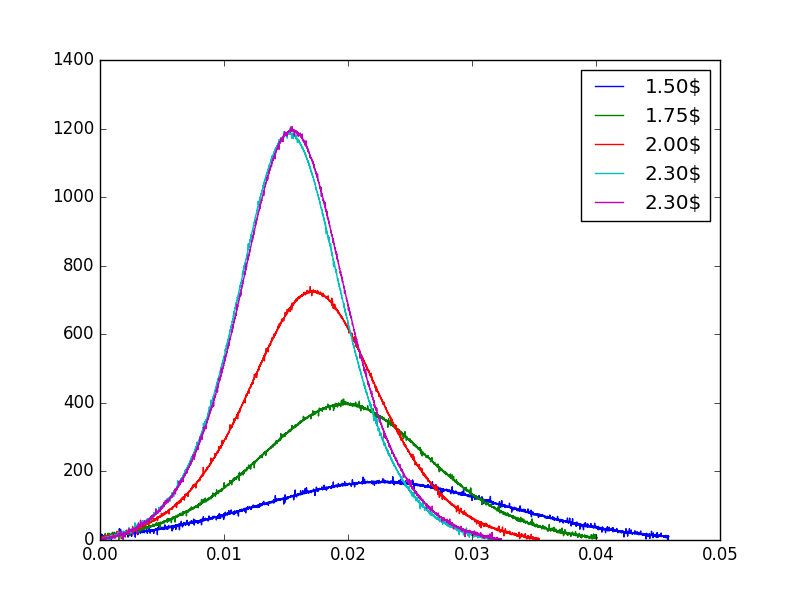
\includegraphics[height=0.4\textheight]{fig02/power.png}
	\mycaption[Pulses of the GSTR]{Pulses of the GSTR.}
	\label{fig:power}
\end{figure}


The neutron lifetime is computed by using the full-width at half maximum values, obtained from the data. Table~\ref{tab:lifetime} gives the results for various prompr criticality insertion values. The approximate value used is 38 $\micro s$, which seems correct for low prompt reactivity insertion, and thus for critical states. However, the higher the prompt reactivity insertion, the higher the neutron lifetime observed.

\begin{table}[!htb]
    \centering
\begin{tabular}{cc}
Prompt reactivity insertion ($\$$) & Neutron lifetime $l (\micro s)$ \\ \hline\hline
1.5 & 39.98 \\
1.75 & 44.28 \\
2.0 & 45.99 \\
2.3 & 49.30 \\
2.3 & 48.55
\end{tabular}
        \caption{Neutron lifetime for various prompt reactivity insertion}\label{tab:lifetime}
\end{table}

The negative temperature coefficient can be computed from the average change in temperature in the core and the prompt reactivity inserted. The average core temperature is obtained by approximation on the peak fuel temperature, considering a factor two between the peak factor and the average, hence a perfect temperature gradient in the core. The values obtained are presented in table~\ref{tab:ntc}, with an average of $9.3 * 10^{-5}$. This is quite far from the approximation from equation~\ref{eqa}, with an error between 15 and 35\%.

We can see on figure~\ref{fig:alpha} that the negative temperature coefficient varies linearly with the average core temperature, with a $R^2$ value of 0.998.

\begin{equation}{\label{eqa1}}
\alpha = 4.38 * 10^{-5} + 3.486 * 10^{-7}(\bar{T}-T_{ini})
\end{equation}

\begin{table}[!htb]
    \centering
\begin{tabular}{cccc}
Prompt reactivity insertion ($\$$) & Average $\Delta T$ (Celsius) & $\alpha$ $(\$/Celsius)$ & Estimate \\ \hline\hline
1.5 & 92.7 & $7.5 * 10^{-5}$ & $1.17 * 10^{-4}$ \\
1.75 & 120.8 & $8.7 * 10^{-5}$ & $1.20 * 10^{-4}$ \\
2.0 & 147.2 & $9.5 * 10^{-5}$  & $1.22 * 10^{-4}$ \\
2.3 & 174.5 & $1.0 * 10^{-4}$  & $1.24 * 10^{-4}$ \\
2.3 & 174.2 & $1.0 * 10^{-4}$ & $1.24 * 10^{-4}$
\end{tabular}
        \caption{Negative temperature coefficient for various prompt reactivity insertion}\label{tab:ntc}
\end{table}


\begin{figure}[t!]
	\centering
	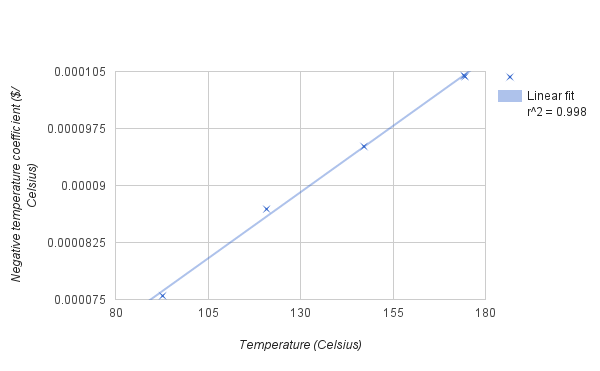
\includegraphics[height=0.4\textheight]{fig02/alpha.png}
	\mycaption[Negative temperature coefficient vs temperature]{Negative temperature coefficient vs temperature.}
	\label{fig:alpha}
\end{figure}


The specific heat of the core can also be measured for various prompt reactivity insertion following Fuchs-Nordheim model. Table~\ref{tab:cp} shows the results, with an error between 2 and 8\% between the measured value and the estimate, the measured value using the average negative temperature coefficient calculated previously.

\begin{table}[!htb]
    \centering
\begin{tabular}{ccc}
Prompt reactivity insertion ($\$$) & Specific heat of the core ($W.s/Celsius$) & Estimate \\ \hline\hline
1.5 & 112280 & 109657 \\
1.75 & 123245 & 114855 \\
2.0 & 129377  & 119724 \\
2.3 & 133916  & 124774 \\
2.3 & 131243  & 124731
\end{tabular}
        \caption{Specific heat of the core for various prompt reactivity insertion}\label{tab:cp}
\end{table}


\begin{figure}[t!]
	\centering
	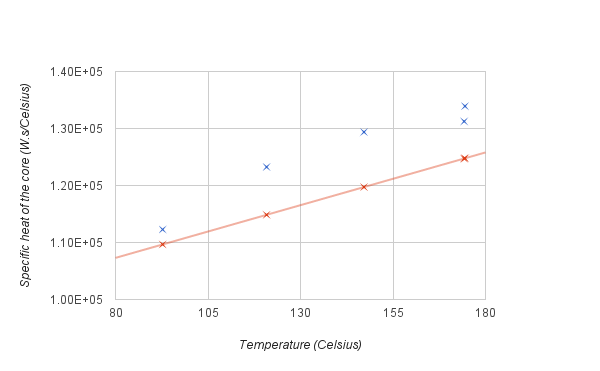
\includegraphics[height=0.4\textheight]{fig02/cp.png}
	\mycaption[Total heat of the core vs temperature]{Total heat of the core vs temperature.}
	\label{fig:cp}
\end{figure}

It is possible to see on figures~\ref{fig:energy} to~\ref{fig:period} that the experiment agrees with the trend predicted by the Fuchs-Nordheim model. Indeed, the fuel temperature and the pulse energy correlates linearly with the prompt reactivity insertion (respectively $R^2 = 0.998$ and $R^2 = 0.999$). Moreover, the inverse dependance of the FWHM and the pulse period with the prompt reactivity insertion is confirmed.

The peak power also clearly shows a second degree polynomial trend, on figure~\ref{fig:power}.


\section{Uncertainties}

Several uncertainty sources must be considered. First and foremost, the prompt reactivity insertion is estimated through the use of the calibration curves. In that regards, the uncertainties observed when calculating this curve propagates here. In the case of the GSTR, it has been shown that the transient rod might be slightly off-centered, skewed toward the top of the core~\cite{lher01}.

A telling way to obtain parts of the uncertainties in the system is to compare the two measurement made for a maximum pulse, with a \$2.3 prompt reactivity insertion. One can see that even though the conditions are supposed to be identical, some differences can be observed. Indeed, table~\ref{tab:comp} presents the relative errors.

\begin{table}[!htb]
    \centering
\begin{tabular}{p{6cm}c}
Parameter & Relative difference \\ \hline\hline
Reactivity & 0\% \\
FWHM & 1.5\% \\
Pulse energy & 2.3\% \\
Pulse period & 1.7\% \\
Fuel temperature peak & 0.3\% \\
\hline
Neutron lifetime & 1.5\% \\
Specific core heat & 2.3\% \\
Prompt negative temperature coefficient & -0.3\%
\end{tabular}
        \caption{Relative difference between the different parameters for identical prompt reactivity insertion}\label{tab:comp}
\end{table}

This table does not represent all the uncertainties in the system, it merely illustrates a potential impact. It is however useful to give us an idea of the uncertainties of the measurements.

One can see then that the estimates for $\alpha$ and $C$ are not very precise, and could gain to be calculated again, using figures~\ref{fig:alpha} and~\ref{fig:cp}.
